\documentclass[]{article}
\usepackage{lmodern}
\usepackage{amssymb,amsmath}
\usepackage{ifxetex,ifluatex}
\usepackage{fixltx2e} % provides \textsubscript
\ifnum 0\ifxetex 1\fi\ifluatex 1\fi=0 % if pdftex
  \usepackage[T1]{fontenc}
  \usepackage[utf8]{inputenc}
\else % if luatex or xelatex
  \ifxetex
    \usepackage{mathspec}
    \usepackage{xltxtra,xunicode}
  \else
    \usepackage{fontspec}
  \fi
  \defaultfontfeatures{Mapping=tex-text,Scale=MatchLowercase}
  \newcommand{\euro}{€}
\fi
% use upquote if available, for straight quotes in verbatim environments
\IfFileExists{upquote.sty}{\usepackage{upquote}}{}
% use microtype if available
\IfFileExists{microtype.sty}{%
\usepackage{microtype}
\UseMicrotypeSet[protrusion]{basicmath} % disable protrusion for tt fonts
}{}
\usepackage[margin=1in]{geometry}
\usepackage{color}
\usepackage{fancyvrb}
\newcommand{\VerbBar}{|}
\newcommand{\VERB}{\Verb[commandchars=\\\{\}]}
\DefineVerbatimEnvironment{Highlighting}{Verbatim}{commandchars=\\\{\}}
% Add ',fontsize=\small' for more characters per line
\usepackage{framed}
\definecolor{shadecolor}{RGB}{248,248,248}
\newenvironment{Shaded}{\begin{snugshade}}{\end{snugshade}}
\newcommand{\KeywordTok}[1]{\textcolor[rgb]{0.13,0.29,0.53}{\textbf{{#1}}}}
\newcommand{\DataTypeTok}[1]{\textcolor[rgb]{0.13,0.29,0.53}{{#1}}}
\newcommand{\DecValTok}[1]{\textcolor[rgb]{0.00,0.00,0.81}{{#1}}}
\newcommand{\BaseNTok}[1]{\textcolor[rgb]{0.00,0.00,0.81}{{#1}}}
\newcommand{\FloatTok}[1]{\textcolor[rgb]{0.00,0.00,0.81}{{#1}}}
\newcommand{\CharTok}[1]{\textcolor[rgb]{0.31,0.60,0.02}{{#1}}}
\newcommand{\StringTok}[1]{\textcolor[rgb]{0.31,0.60,0.02}{{#1}}}
\newcommand{\CommentTok}[1]{\textcolor[rgb]{0.56,0.35,0.01}{\textit{{#1}}}}
\newcommand{\OtherTok}[1]{\textcolor[rgb]{0.56,0.35,0.01}{{#1}}}
\newcommand{\AlertTok}[1]{\textcolor[rgb]{0.94,0.16,0.16}{{#1}}}
\newcommand{\FunctionTok}[1]{\textcolor[rgb]{0.00,0.00,0.00}{{#1}}}
\newcommand{\RegionMarkerTok}[1]{{#1}}
\newcommand{\ErrorTok}[1]{\textbf{{#1}}}
\newcommand{\NormalTok}[1]{{#1}}
\usepackage{graphicx}
\makeatletter
\def\maxwidth{\ifdim\Gin@nat@width>\linewidth\linewidth\else\Gin@nat@width\fi}
\def\maxheight{\ifdim\Gin@nat@height>\textheight\textheight\else\Gin@nat@height\fi}
\makeatother
% Scale images if necessary, so that they will not overflow the page
% margins by default, and it is still possible to overwrite the defaults
% using explicit options in \includegraphics[width, height, ...]{}
\setkeys{Gin}{width=\maxwidth,height=\maxheight,keepaspectratio}
\ifxetex
  \usepackage[setpagesize=false, % page size defined by xetex
              unicode=false, % unicode breaks when used with xetex
              xetex]{hyperref}
\else
  \usepackage[unicode=true]{hyperref}
\fi
\hypersetup{breaklinks=true,
            bookmarks=true,
            pdfauthor={},
            pdftitle={},
            colorlinks=true,
            citecolor=blue,
            urlcolor=blue,
            linkcolor=magenta,
            pdfborder={0 0 0}}
\urlstyle{same}  % don't use monospace font for urls
\setlength{\parindent}{0pt}
\setlength{\parskip}{6pt plus 2pt minus 1pt}
\setlength{\emergencystretch}{3em}  % prevent overfull lines
\setcounter{secnumdepth}{0}

%%% Use protect on footnotes to avoid problems with footnotes in titles
\let\rmarkdownfootnote\footnote%
\def\footnote{\protect\rmarkdownfootnote}

%%% Change title format to be more compact
\usepackage{titling}

% Create subtitle command for use in maketitle
\newcommand{\subtitle}[1]{
  \posttitle{
    \begin{center}\large#1\end{center}
    }
}

\setlength{\droptitle}{-2em}
  \title{}
  \pretitle{\vspace{\droptitle}}
  \posttitle{}
  \author{}
  \preauthor{}\postauthor{}
  \date{}
  \predate{}\postdate{}



\begin{document}

\maketitle


\section{Statistical Inference}\label{statistical-inference}

\subsubsection{Course Project 1:
CP1\_template}\label{course-project-1-cp1ux5ftemplate}

\subsubsection{Introduction}\label{introduction}

This document presents the results of the Course Project for the
Coursera course: Statistical Inference. This assessment makes use of
simulation techniques in order to explore inference and do some simple
inferential data analysis.

The student is to investigate the exponential distribution in R and to
draw comparison against the Central Limit Theorem. The exponential
distribution can be simulated in R with rexp(n, lambda) where lambda is
the rate parameter. The mean of exponential distribution is 1/lambda and
the standard deviation is also 1/lambda.

The student is to investigate the distribution of averages of 40
exponentials, with a thousand simulations.

\subsubsection{1. Load Packages}\label{load-packages}

\begin{Shaded}
\begin{Highlighting}[]
\NormalTok{for (package in }\KeywordTok{c}\NormalTok{(}\StringTok{'ggplot2'}\NormalTok{)) \{}
 
    \NormalTok{if (!}\KeywordTok{require}\NormalTok{(package, }\DataTypeTok{character.only =} \OtherTok{TRUE}\NormalTok{, }\DataTypeTok{quietly =} \OtherTok{FALSE}\NormalTok{)) \{}
        \KeywordTok{install.packages}\NormalTok{(package)}
        \KeywordTok{library}\NormalTok{(package, }\DataTypeTok{character.only =} \OtherTok{TRUE}\NormalTok{)}
    \NormalTok{\}}
\NormalTok{\}}
\end{Highlighting}
\end{Shaded}

\subsubsection{2. Simulations}\label{simulations}

Set lambda for exponential function, number of exponentials and numbers
of sample/tests.

\begin{Shaded}
\begin{Highlighting}[]
\KeywordTok{set.seed}\NormalTok{(}\DecValTok{123456789}\NormalTok{)}

\NormalTok{val_lambda <-}\StringTok{ }\FloatTok{0.2}
\NormalTok{val_n <-}\StringTok{ }\DecValTok{40}
\NormalTok{val_sims <-}\StringTok{ }\DecValTok{1000}
\end{Highlighting}
\end{Shaded}

Run sample/tests.

\begin{Shaded}
\begin{Highlighting}[]
\NormalTok{data_expdist <-}\StringTok{ }\KeywordTok{data.frame}\NormalTok{(}\DataTypeTok{means =} \DecValTok{1}\NormalTok{:val_sims)}

\NormalTok{for (i in }\DecValTok{1}\NormalTok{:val_sims) \{}
 
  \NormalTok{val_sim <-}\StringTok{ }\KeywordTok{rexp}\NormalTok{(val_n, val_lambda)}
  \NormalTok{data_expdist[i, }\DecValTok{1}\NormalTok{] <-}\StringTok{ }\KeywordTok{mean}\NormalTok{(val_sim)}
 
\NormalTok{\}}

\KeywordTok{remove}\NormalTok{(val_sim)}
\end{Highlighting}
\end{Shaded}

Find range and plot sampled data.

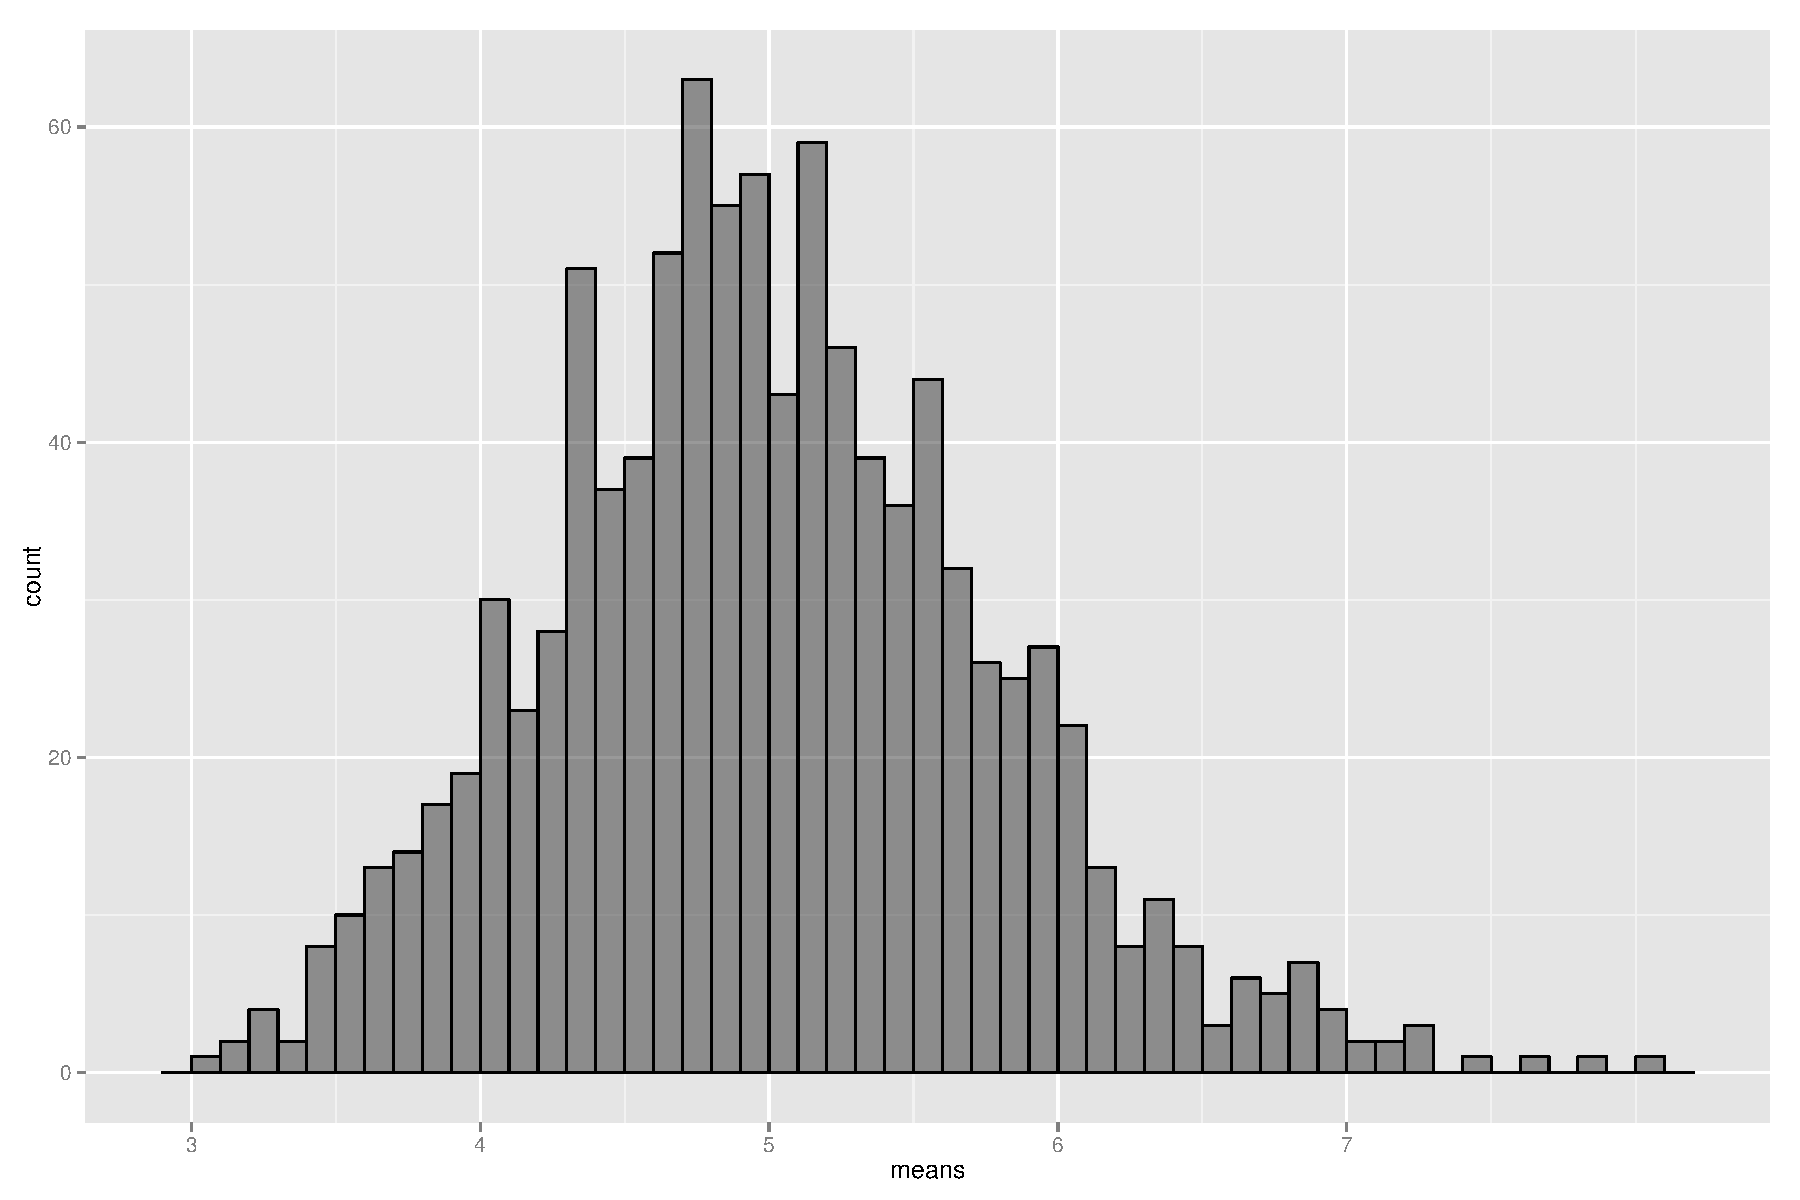
\includegraphics{figure/unnamed-chunk-4-1.pdf}

\subsubsection{3. Sample Mean vs.~Theoretical
Mean}\label{sample-mean-vs.theoretical-mean}

Find the theoretical mean of the exponential distribution

\begin{Shaded}
\begin{Highlighting}[]
\NormalTok{val_truemu <-}\StringTok{ }\DecValTok{1}\NormalTok{/val_lambda}
\NormalTok{val_truemu}
\end{Highlighting}
\end{Shaded}

\begin{verbatim}
## [1] 5
\end{verbatim}

Find the mean of the sampled distribution

\begin{Shaded}
\begin{Highlighting}[]
\NormalTok{val_samplemu <-}\StringTok{ }\KeywordTok{mean}\NormalTok{(data_expdist$means)}
\NormalTok{val_samplemu}
\end{Highlighting}
\end{Shaded}

\begin{verbatim}
## [1] 5.005439
\end{verbatim}

\subsubsection{4. Sample Variance vs.~Theoretical
Variance}\label{sample-variance-vs.theoretical-variance}

Find the theoretical variance of the exponential distribution

\begin{Shaded}
\begin{Highlighting}[]
\NormalTok{val_truevar <-}\StringTok{ }\NormalTok{(}\DecValTok{1}\NormalTok{/val_lambda/}\KeywordTok{sqrt}\NormalTok{(val_n))^}\DecValTok{2}
\NormalTok{val_truevar}
\end{Highlighting}
\end{Shaded}

\begin{verbatim}
## [1] 0.625
\end{verbatim}

Find the variance of the sampled distribution

\begin{Shaded}
\begin{Highlighting}[]
\NormalTok{val_samplevar <-}\StringTok{ }\KeywordTok{var}\NormalTok{(data_expdist$means)}
\NormalTok{val_samplevar}
\end{Highlighting}
\end{Shaded}

\begin{verbatim}
## [1] 0.6010095
\end{verbatim}

\subsubsection{5. Distribution}\label{distribution}

Plot sampled means against true mean distribution

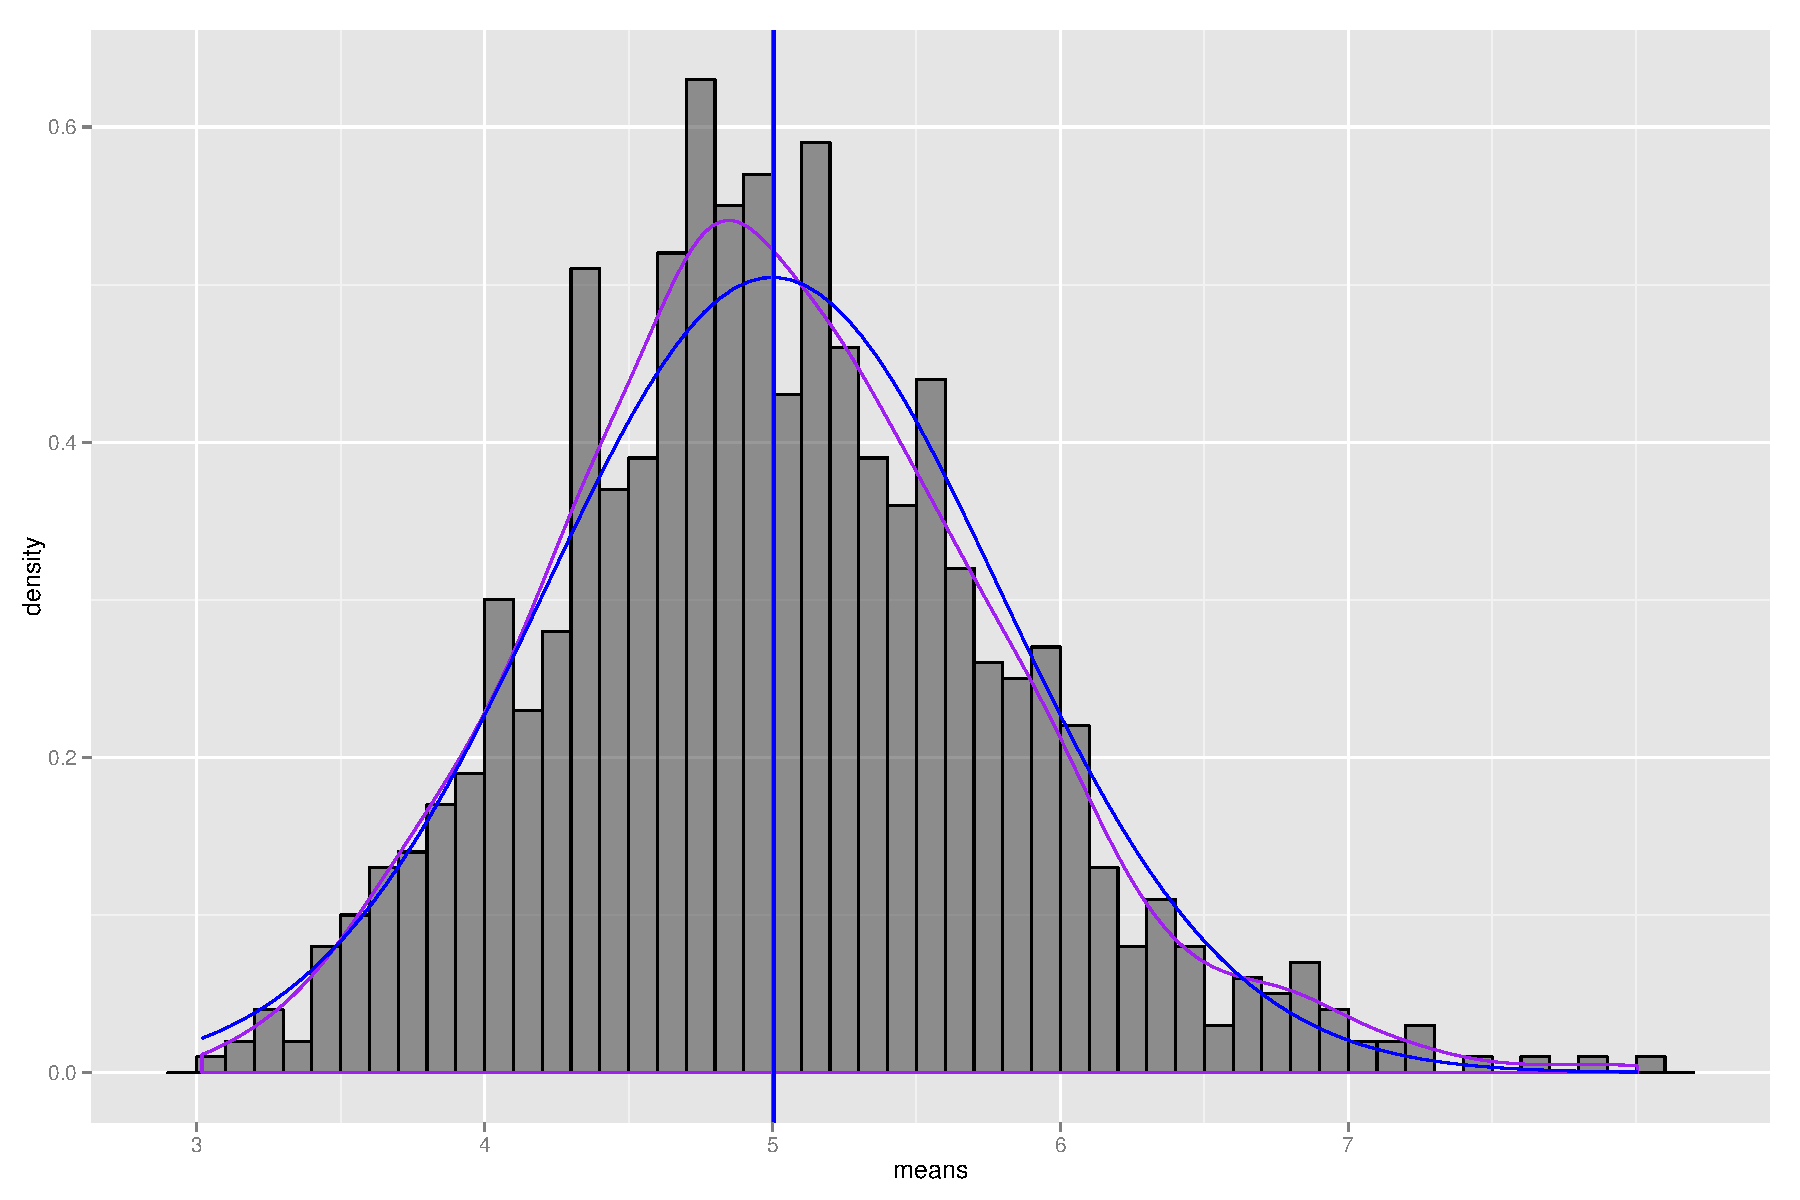
\includegraphics{figure/unnamed-chunk-9-1.pdf}

Evaluate the coverage of confidence intervals for a standard normal
distribution:

\begin{Shaded}
\begin{Highlighting}[]
  \KeywordTok{mean}\NormalTok{(data_expdist$means) +}\StringTok{ }\KeywordTok{c}\NormalTok{(-}\DecValTok{1}\NormalTok{,}\DecValTok{1}\NormalTok{) *}\StringTok{ }\FloatTok{1.96} \NormalTok{*}\StringTok{ }\KeywordTok{sd}\NormalTok{(data_expdist$means)/}\KeywordTok{sqrt}\NormalTok{(}\KeywordTok{nrow}\NormalTok{(data_expdist))}
\end{Highlighting}
\end{Shaded}

\begin{verbatim}
## [1] 4.957389 5.053490
\end{verbatim}

\end{document}
